\documentclass[a4paper]{book}
\usepackage{a4wide}
\usepackage{makeidx}
\usepackage{fancyhdr}
\usepackage{graphicx}
\usepackage{multicol}
\usepackage{float}
\usepackage{alltt}
\usepackage{times}
\ifx\pdfoutput\undefined
\usepackage[ps2pdf,
            pagebackref=true,
            colorlinks=true,
            linkcolor=blue
           ]{hyperref}
\else
\usepackage[pdftex,
            pagebackref=true,
            colorlinks=true,
            linkcolor=blue
           ]{hyperref}
\fi
\usepackage{doxygen}
\makeindex
\setcounter{tocdepth}{1}
\setlength{\footrulewidth}{0.4pt}
\begin{document}
\begin{titlepage}
\vspace*{7cm}
\begin{center}
{\Large Sample Reference Manual}\\
\vspace*{1cm}
{\large Generated by Doxygen 1.2.18}\\
\vspace*{0.5cm}
{\small Tue Sep 16 20:42:20 2003}\\
\end{center}
\end{titlepage}
\clearemptydoublepage
\pagenumbering{roman}
\tableofcontents
\clearemptydoublepage
\pagenumbering{arabic}
\chapter{Sample documentation example}
\label{index}\hypertarget{index}{}

\hypertarget{intro}{}\subsection{Introduction}\label{intro}


This tutorial is a simple example of most of the features you will be using in doxygen. There are many more, but these are the most useful. Next see how you can use this yourself. \hyperlink{own}{Your own documentation}


\chapter{Sample Module Index}
\section{Sample Modules}
Here is a list of all modules:\begin{CompactList}
\item \contentsline{section}{Stack}{\pageref{group__stack}}{}
\end{CompactList}

\chapter{Sample Data Structure Index}
\section{Sample Data Structures}
Here are the data structures with brief descriptions:\begin{CompactList}
\item\contentsline{section}{\hyperlink{structstack}{stack} (This is a stack struct)}{\pageref{structstack}}{}
\end{CompactList}

\chapter{Sample File Index}
\section{Sample File List}
Here is a list of all documented files with brief descriptions:\begin{CompactList}
\item\contentsline{section}{{\bf documentation.h} }{\pageref{documentation_8h}}{}
\item\contentsline{section}{\hyperlink{stack_8c}{stack.c} }{\pageref{stack_8c}}{}
\item\contentsline{section}{\hyperlink{stack_8h}{stack.h} (This is brief description of this file)}{\pageref{stack_8h}}{}
\end{CompactList}

\chapter{Sample Page Index}
\section{Sample Related Pages}
Here is a list of all related documentation pages:\begin{CompactList}
\item \contentsline{section}{Your own documentation}{\pageref{own}}{}

\item \contentsline{section}{Todo List}{\pageref{todo}}{}

\item \contentsline{section}{Deprecated List}{\pageref{deprecated}}{}

\item \contentsline{section}{Bug List}{\pageref{bug}}{}

\end{CompactList}

\chapter{Sample Module Documentation}
\hypertarget{group__stack}{
\section{Stack}
\label{group__stack}\index{Stack@{Stack}}
}
\subsection*{Data Structures}
\begin{CompactItemize}
\item 
struct \hyperlink{structstack}{stack}
\begin{CompactList}\small\item\em This is a stack struct.\item\end{CompactList}\end{CompactItemize}
\subsection*{Functions}
\begin{CompactItemize}
\item 
int \hyperlink{group__stack_a0}{push} (\hyperlink{structstack}{stack} s, int val)
\begin{CompactList}\small\item\em This function is used to push stuff.\item\end{CompactList}\item 
int \hyperlink{group__stack_a1}{pop} (\hyperlink{structstack}{stack} s)
\begin{CompactList}\small\item\em This pops.\item\end{CompactList}\item 
int \hyperlink{group__stack_a2}{top} (\hyperlink{structstack}{stack} s)
\begin{CompactList}\small\item\em Take a look at the top.\item\end{CompactList}\end{CompactItemize}


\subsection{Function Documentation}
\hypertarget{group__stack_a1}{
\index{Stack@{Stack}!pop@{pop}}
\index{pop@{pop}!Stack@{Stack}}
\subsubsection[pop]{\setlength{\rightskip}{0pt plus 5cm}int pop (\hyperlink{structstack}{stack} {\em s})}}
\label{group__stack_a1}


This pops.

It is used to pop stuff

\begin{Desc}
\item[Warning: ]\par
This can give you an error if there is nothing to pop \end{Desc}
\begin{Desc}
\item[See also: ]\par
stack , push \end{Desc}
\begin{Desc}
\item[Parameters: ]\par
\begin{description}
\item[{\em 
s}]the stack to get an element from\end{description}
\end{Desc}
\begin{Desc}
\item[Returns: ]\par
\end{Desc}
\hypertarget{group__stack_a0}{
\index{Stack@{Stack}!push@{push}}
\index{push@{push}!Stack@{Stack}}
\subsubsection[push]{\setlength{\rightskip}{0pt plus 5cm}int push (\hyperlink{structstack}{stack} {\em s}, int {\em val})}}
\label{group__stack_a0}


This function is used to push stuff.

It puts stuff on the end.

\begin{Desc}
\item[\hyperlink{bug__bug000001}{Bug: }]\par
this function rules too much\end{Desc}
 \begin{Desc}
\item[Parameters: ]\par
\begin{description}
\item[{\em 
s}]This is the stack to push onto \item[{\em 
val}]This is the value to push\end{description}
\end{Desc}
\begin{Desc}
\item[Returns: ]\par
\begin{CompactItemize}
\item 
a non-negative value indicates success\item 
a negative return value indicates that the push was not successful\item 
The - creates a bullet list \end{CompactItemize}
\end{Desc}
\begin{Desc}
\item[Examples: ]\par
\hyperlink{stack__example_8c-example}{stack\_\-example.c}.\end{Desc}


Definition at line 13 of file stack.c.

References stack::end, and stack::stack.\hypertarget{group__stack_a2}{
\index{Stack@{Stack}!top@{top}}
\index{top@{top}!Stack@{Stack}}
\subsubsection[top]{\setlength{\rightskip}{0pt plus 5cm}int top (\hyperlink{structstack}{stack} {\em s})}}
\label{group__stack_a2}


Take a look at the top.

This is another way to do documentation. It is better to put the documentation in the source, because then you can edit them together.

\begin{Desc}
\item[Returns: ]\par
The top of the stack \end{Desc}

\chapter{Sample Data Structure Documentation}
\hypertarget{structstack}{
\section{stack Struct Reference}
\label{structstack}\index{stack@{stack}}
}
This is a stack struct. 


{\tt \#include $<$stack.h$>$}

\subsection*{Data Fields}
\begin{CompactItemize}
\item 
int \hyperlink{structstack_m0}{start}
\begin{CompactList}\small\item\em This is the start of the stack.\item\end{CompactList}\item 
\hypertarget{structstack_m1}{
\index{end@{end}!stack@{stack}}\index{stack@{stack}!end@{end}}
int \hyperlink{structstack_m1}{end}}
\label{structstack_m1}

\begin{CompactList}\small\item\em There are automatically brief descriptions.\item\end{CompactList}\item 
int \hyperlink{structstack_m2}{stack} \mbox{[}100\mbox{]}
\begin{CompactList}\small\item\em This is the data of the stack. This is a second line of brief description.\item\end{CompactList}\item 
\hypertarget{structstack_m3}{
\index{id@{id}!stack@{stack}}\index{stack@{stack}!id@{id}}
int \hyperlink{structstack_m3}{id}}
\label{structstack_m3}

\begin{CompactList}\small\item\em ID number.\item\end{CompactList}\item 
void $\ast$($\ast$ \hyperlink{structstack_m4}{helper} )(int, int, char $\ast$)
\end{CompactItemize}


\subsection{Detailed Description}
This is a stack struct.

It does stack stuff \begin{Desc}
\item[Author: ]\par
ME \end{Desc}
\begin{Desc}
\item[Examples: ]\par


\hyperlink{stack__example_8c-example}{stack\_\-example.c}.\end{Desc}




Definition at line 49 of file stack.h.

\subsection{Field Documentation}
\hypertarget{structstack_m4}{
\index{stack@{stack}!helper@{helper}}
\index{helper@{helper}!stack@{stack}}
\subsubsection[helper]{\setlength{\rightskip}{0pt plus 5cm}void$\ast$($\ast$ stack::helper)(int, int, char $\ast$)}}
\label{structstack_m4}


It handles these good too.  This is a pointer to a function that takes 2 ints and a char $\ast$  and returns a void $\ast$ \hypertarget{structstack_m2}{
\index{stack@{stack}!stack@{stack}}
\index{stack@{stack}!stack@{stack}}
\subsubsection[stack]{\setlength{\rightskip}{0pt plus 5cm}int stack::stack\mbox{[}100\mbox{]}}}
\label{structstack_m2}


This is the data of the stack. This is a second line of brief description.

If you do it this way, they dont only have to be brief descriptions 

Definition at line 62 of file stack.h.

Referenced by push().\hypertarget{structstack_m0}{
\index{stack@{stack}!start@{start}}
\index{start@{start}!stack@{stack}}
\subsubsection[start]{\setlength{\rightskip}{0pt plus 5cm}int stack::start}}
\label{structstack_m0}


This is the start of the stack.

and multiline too, with details. 

Definition at line 51 of file stack.h.

The documentation for this struct was generated from the following file:\begin{CompactItemize}
\item 
\hyperlink{stack_8h}{stack.h}\end{CompactItemize}

\chapter{Sample File Documentation}
\hypertarget{stack_8c}{
\section{stack.c File Reference}
\label{stack_8c}\index{stack.c@{stack.c}}
}
{\tt \#include \char`\"{}stack.h\char`\"{}}\par


Include dependency graph for stack.c:\begin{figure}[H]
\begin{center}
\leavevmode
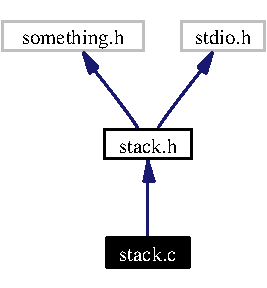
\includegraphics[width=81pt]{stack_8c__incl}
\end{center}
\end{figure}
\subsection*{Functions}
\begin{CompactItemize}
\item 
int \hyperlink{group__stack_a0}{push} (\hyperlink{structstack}{stack} s, int val)
\begin{CompactList}\small\item\em This function is used to push stuff.\item\end{CompactList}\item 
int \hyperlink{stack_8c_a1}{pop} (\hyperlink{structstack}{stack} s, int val)
\end{CompactItemize}


\subsection{Detailed Description}




Definition in file \hyperlink{stack_8c-source}{stack.c}.

\subsection{Function Documentation}
\hypertarget{stack_8c_a1}{
\index{stack.c@{stack.c}!pop@{pop}}
\index{pop@{pop}!stack.c@{stack.c}}
\subsubsection[pop]{\setlength{\rightskip}{0pt plus 5cm}int pop (\hyperlink{structstack}{stack} {\em s}, int {\em val})}}
\label{stack_8c_a1}


\begin{Desc}
\item[\hyperlink{todo__todo000001}{Todo: }]\par
 Impliment this function \end{Desc}
 \begin{Desc}
\item[Examples: ]\par
\hyperlink{stack__example_8c-example}{stack\_\-example.c}.\end{Desc}


Definition at line 24 of file stack.c.
\hypertarget{stack_8h}{
\section{stack.h File Reference}
\label{stack_8h}\index{stack.h@{stack.h}}
}
This is brief description of this file. 


{\tt \#include \char`\"{}something.h\char`\"{}}\par
{\tt \#include $<$stdio.h$>$}\par


Include dependency graph for stack.h:\begin{figure}[H]
\begin{center}
\leavevmode
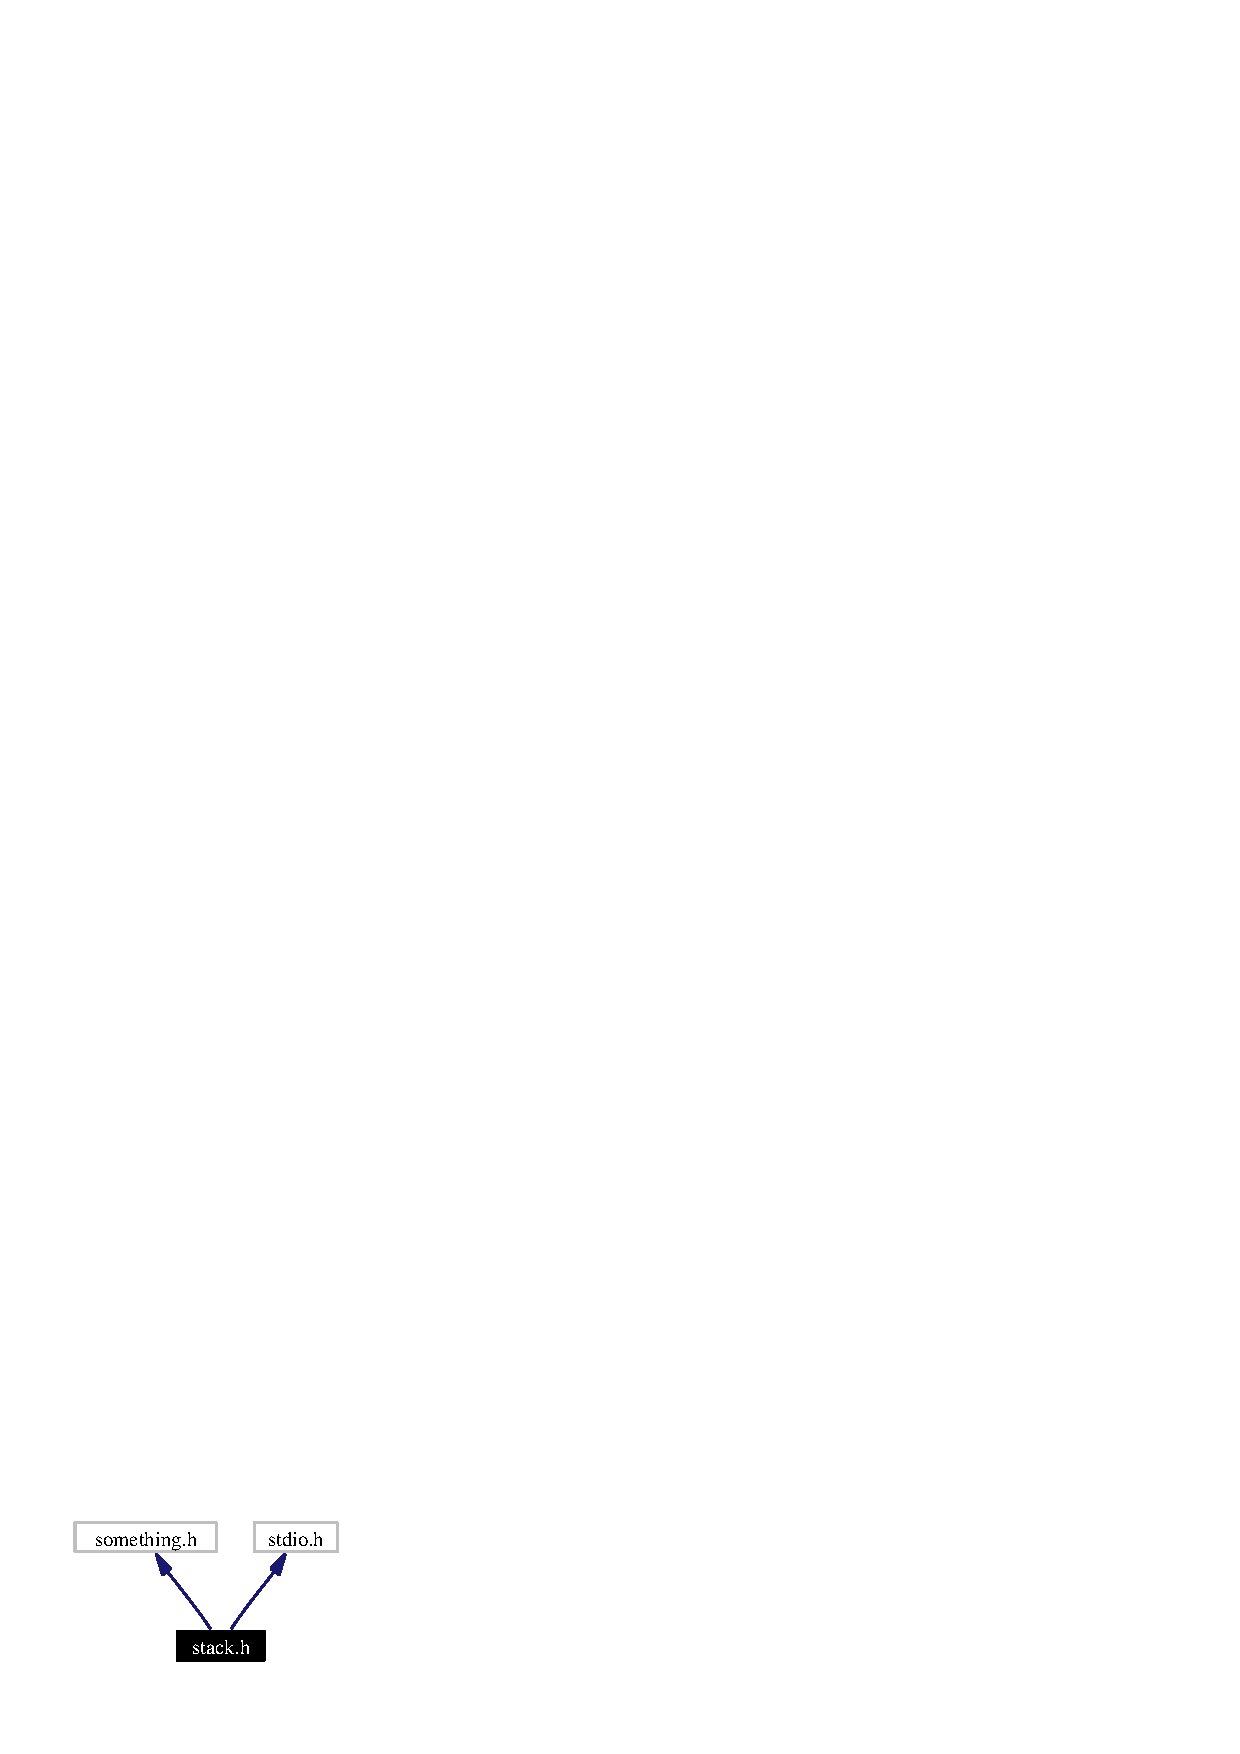
\includegraphics[width=81pt]{stack_8h__incl}
\end{center}
\end{figure}


This graph shows which files directly or indirectly include this file:\begin{figure}[H]
\begin{center}
\leavevmode
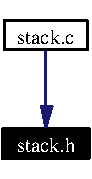
\includegraphics[width=39pt]{stack_8h__dep__incl}
\end{center}
\end{figure}
\subsection*{Data Structures}
\begin{CompactItemize}
\item 
struct \hyperlink{structstack}{stack}
\begin{CompactList}\small\item\em This is a stack struct.\item\end{CompactList}\end{CompactItemize}
\subsection*{Defines}
\begin{CompactItemize}
\item 
\#define \hyperlink{stack_8h_a0}{ENOMEM}\ -1
\item 
\hypertarget{stack_8h_a1}{
\index{EXAMPLE@{EXAMPLE}!stack.h@{stack.h}}\index{stack.h@{stack.h}!EXAMPLE@{EXAMPLE}}
\#define \hyperlink{stack_8h_a1}{EXAMPLE}\ -2}
\label{stack_8h_a1}

\begin{CompactList}\small\item\em you may also only have one line of comments\item\end{CompactList}\item 
\hypertarget{stack_8h_a2}{
\index{EXAMPLE2@{EXAMPLE2}!stack.h@{stack.h}}\index{stack.h@{stack.h}!EXAMPLE2@{EXAMPLE2}}
\#define \hyperlink{stack_8h_a2}{EXAMPLE2}\ -3}
\label{stack_8h_a2}

\begin{CompactList}\small\item\em This is how you put documentation after the fact.\item\end{CompactList}\end{CompactItemize}
\subsection*{Functions}
\begin{CompactItemize}
\item 
int \hyperlink{stack_8h_a3}{push} (\hyperlink{structstack}{stack} s, int val)
\begin{CompactList}\small\item\em This function is used to push stuff.\item\end{CompactList}\item 
int \hyperlink{group__stack_a1}{pop} (\hyperlink{structstack}{stack} s)
\begin{CompactList}\small\item\em This pops.\item\end{CompactList}\item 
int \hyperlink{stack_8h_a5}{get\_\-elem} (\hyperlink{structstack}{stack} s, int val)
\begin{CompactList}\small\item\em This gets an element.\item\end{CompactList}\item 
int \hyperlink{group__stack_a2}{top} (\hyperlink{structstack}{stack} s)
\begin{CompactList}\small\item\em Take a look at the top.\item\end{CompactList}\end{CompactItemize}


\subsection{Detailed Description}
This is brief description of this file.

 This is a slightly longer description of the file. Also note that the 'backslash'file command is needed or doxygen wont pull any declarations from the file \begin{Desc}
\item[Version: ]\par
a million \end{Desc}
\begin{Desc}
\item[Author: ]\par
someone without much to do , some other guy too \end{Desc}
\begin{Desc}
\item[Date: ]\par
1896-2430\end{Desc}


Definition in file \hyperlink{stack_8h-source}{stack.h}.

\subsection{Define Documentation}
\hypertarget{stack_8h_a0}{
\index{stack.h@{stack.h}!ENOMEM@{ENOMEM}}
\index{ENOMEM@{ENOMEM}!stack.h@{stack.h}}
\subsubsection[ENOMEM]{\setlength{\rightskip}{0pt plus 5cm}\#define ENOMEM\ -1}}
\label{stack_8h_a0}


This describes this define and what it is used for.  In this case it is used to say there is no memory.  These are automatically brief descriptions 

Definition at line 29 of file stack.h.

\subsection{Function Documentation}
\hypertarget{stack_8h_a5}{
\index{stack.h@{stack.h}!get_elem@{get\_\-elem}}
\index{get_elem@{get\_\-elem}!stack.h@{stack.h}}
\subsubsection[get\_\-elem]{\setlength{\rightskip}{0pt plus 5cm}int get\_\-elem (\hyperlink{structstack}{stack} {\em s}, int {\em val})}}
\label{stack_8h_a5}


This gets an element.

It is used to get stuff

\begin{Desc}
\item[\hyperlink{deprecated__deprecated000001}{Deprecated: }]\par
Dont use this anymore, for various reasons\end{Desc}
 \begin{Desc}
\item[Parameters: ]\par
\begin{description}
\item[{\em 
s}]stack to get item from \item[{\em 
i}]This is the index\end{description}
\end{Desc}
\begin{Desc}
\item[Returns: ]\par
\end{Desc}
\hypertarget{stack_8h_a3}{
\index{stack.h@{stack.h}!push@{push}}
\index{push@{push}!stack.h@{stack.h}}
\subsubsection[push]{\setlength{\rightskip}{0pt plus 5cm}int push (\hyperlink{structstack}{stack} {\em s}, int {\em val})}}
\label{stack_8h_a3}


This function is used to push stuff.

It puts stuff on the end.

\begin{Desc}
\item[\hyperlink{bug__bug000001}{Bug: }]\par
this function rules too much\end{Desc}
 \begin{Desc}
\item[Parameters: ]\par
\begin{description}
\item[{\em 
s}]This is the stack to push onto \item[{\em 
val}]This is the value to push\end{description}
\end{Desc}
\begin{Desc}
\item[Returns: ]\par
\begin{CompactItemize}
\item 
a non-negative value indicates success\item 
a negative return value indicates that the push was not successful\item 
The - creates a bullet list \end{CompactItemize}
\end{Desc}


Definition at line 13 of file stack.c.

References stack::end, and stack::stack.
\chapter{Sample Example Documentation}
\hypertarget{stack__example_8c-example}{
\section{stack\_\-example.c}
}


This is an example of how to use the stack struct



\footnotesize\begin{verbatim}void main()
{
    stack s;
    int y;
    push(s, 3);
    y = pop(s);  //y will be 3
}
\end{verbatim}\normalsize 

\chapter{Sample Page Documentation}
\hypertarget{own}{}\section{Your own documentation}\label{own}


You just need to start putting these structured comments in your .h files and things will be good.

\hypertarget{own_1}{}\subsection{Step 1: making .h files}\label{own_1}


\hypertarget{own_1_1}{}\subsubsection{Type stuff}\label{own_1_1}


First, type some stuff

\hypertarget{own_1_2}{}\subsubsection{Add documentation}\label{own_1_2}


Then add documentation.

\hypertarget{own_1_3}{}\subsubsection{Compile.}\label{own_1_3}


Then compile


\hypertarget{todo}{}\section{Todo List}\label{todo}
\label{_todo000001}
\hypertarget{todo__todo000001}{}
\begin{description}
\item[Global \hyperlink{stack_8c_a1}{pop}(stack s, int val) ]
 Impliment this function \end{description}
 
\hypertarget{deprecated}{}\section{Deprecated List}\label{deprecated}
\label{_deprecated000001}
\hypertarget{deprecated__deprecated000001}{}
\begin{description}
\item[Global \hyperlink{stack_8h_a5}{get\_\-elem}(stack s, int val) ]
Dont use this anymore, for various reasons\end{description}
 
\hypertarget{bug}{}\section{Bug List}\label{bug}
\label{_bug000001}
\hypertarget{bug__bug000001}{}
\begin{description}
\item[Global \hyperlink{stack_8h_a3}{push}(stack s, int val) ]
this function rules too much\end{description}
 
\printindex
\end{document}
